%\beginsupplement
\section{Supplementary Data}
\label{supplinfo}


\subsection{Potentials}
isoPAHAP tables?
curPAHIP tables?

The atomic coordinates and charges of the minimised 2pent15ring monomer.
Probably should also include the same for corannulene (can pull from CST paper).

\subsection{Dimer energy plots - isoPAHAP potential}

\subsection{Position restraint neglibigility at low temperature}

\subsection{Simulation length equilibration check}
Energies and radial distances don't change significantly when comparing eqm result from 3ns simulation (final 1ns) or 1ns simulation (final 500ps)
Percent error of intermolecular energies are less than 0.2\%
Percent error of radial distances are less than 3.5\%



\subsection{Corannulene crystal structure}
In order to assess / benchmark the structural metrics used in this paper, they have been applied to the known crystal structure of a corannulene. %Further comparison is made with a 2pent15ring system and published large cPAH systems - Actually this should be included in the discussion sections of the paper I think.

X-ray analysis of corannulene was conducted in 1975, and it was determined that the compound crystallises in space group \textit{P}$2_{1}/c$ \cite{hanson1976crystal}.

A crystal structure containing 18 molecules, taken from The Cambridge Crystallographic Data Centre \cite{CORANN11unitcell}, provides an independent verification of the analysis used in this work as well as a known experimental structure useful for comparison.  The crystal density and intermolecular distances are provided in Table \ref{tableSI:crystal}.  Figure XX shows the crystal structure and alignment angles.

% Please add the following required packages to your document preamble:
% \usepackage{multirow}
\begin{table}[]
\begin{tabular}{l|l|l|l|l|l|ll}
\hline
\multicolumn{1}{c|}{\multirow{2}{*}{Cluster}} & \multicolumn{1}{c|}{Diameter} & \multicolumn{1}{c|}{Density} & \multicolumn{1}{c|}{Intermolecular energy} & \multicolumn{1}{c|}{Average intermolecular} & \multicolumn{1}{c|}{Coordination} & \multicolumn{2}{c}{Equilibrium radial distance (nm)} \\ \cline{7-8} 
\multicolumn{1}{c|}{} & \multicolumn{1}{c|}{(nm)} & \multicolumn{1}{c|}{(kg/m3)} & \multicolumn{1}{c|}{(kJ/mol per molecule)} & \multicolumn{1}{c|}{distance (nm)} & \multicolumn{1}{c|}{number} & \multicolumn{1}{c|}{corannulene} & \multicolumn{1}{c}{2pent15ring} \\ \hline
ann\_25 & 2.36 & 1.50 & -75 & 0.59 &  & \multicolumn{1}{l|}{0.86} & -- \\
ann\_40 & 2.77 & 1.49 & -82 & 0.59 &  & \multicolumn{1}{l|}{1.04} & -- \\
ann\_50 & 3.00 & 1.47 & -84 & 0.60 &  & \multicolumn{1}{l|}{1.11} & -- \\
ann\_100 & 3.79 & 1.45 & -92 & 0.59 &  & \multicolumn{1}{l|}{1.42} & -- \\
ann\_200 & 4.79 & 1.45 & -97 & 0.60 &  & \multicolumn{1}{l|}{1.80} & -- \\
two\_25 & 2.96 & 1.59 & -144 & 0.44 &  & \multicolumn{1}{l|}{--} & 1.21 \\
two\_40 & 3.49 & 1.55 & -152 & 0.45 &  & \multicolumn{1}{l|}{--} & 1.37 \\
two\_50 & 3.76 & 1.55 & -157 & 0.45 &  & \multicolumn{1}{l|}{--} & 1.40 \\
two\_100 & 4.77 & 1.52 & -165 & 0.45 &  & \multicolumn{1}{l|}{--} & 1.85 \\
two\_20\_ann\_20 & 3.16 & 1.55 & -125 & 0.44 (0.61/0.43/0.41) &  & \multicolumn{1}{l|}{1.28} & 1.14 \\
two\_50\_ann\_50 & 4.31 & 1.52 & -135 & 0.51 (0.60/0.44/0.47) &  & \multicolumn{1}{l|}{1.83} & 1.50 \\
two\_10\_ann\_30 & 2.98 & 1.52 & -103 & 0.54 (0.58/0.44/0.48) &  & \multicolumn{1}{l|}{1.18} & 0.96 \\
two\_30\_ann\_10 & 3.31 & 1.58 & -147 & 0.44 (0.53/0.43/0.43) &  & \multicolumn{1}{l|}{1.50} & 1.25 \\
two\_40\_K\_1 & 3.50 & 1.48 & -149 & 0.86 &  & \multicolumn{1}{l|}{--} & 1.27 \\
ann\_40\_K\_1 & 2.78 & 1.49 & -88 & 0.67 &  & \multicolumn{1}{l|}{0.99} & -- \\
ann\_40\_K\_2 & 2.79 & 1.54 & -94 & 0.73 &  & \multicolumn{1}{l|}{0.92} & -- \\ \hline
\end{tabular}
\end{table}
%
%(using cut-off value of $R = 0.7$ nm)
%Intermolecular distances: 0.55 nm x 10, 0.61 nm x 6 (for first molecule); 0.61 x 2, 0.72 x 10, 0.73 x 2, 0.76 x 2, 0.78 x 2 (for second molecule), 0.72 x 2, 0.73 x 4, 0.76 x 8, 0.78 x 2, 0.82 x 2 (third molecule)... NOT SURE HOW TO SHOW THESE -> FOLLOW SAME PATTERN USED IN HOW I DISCUSS THIS IN THE PAPER (AVERAGE INTERMOLECULAR DISTS? - WOULD BE 0.57 NM FOR FIRST MOLECULE, ETC)
%
\begin{figure}[!tbh]
\centering
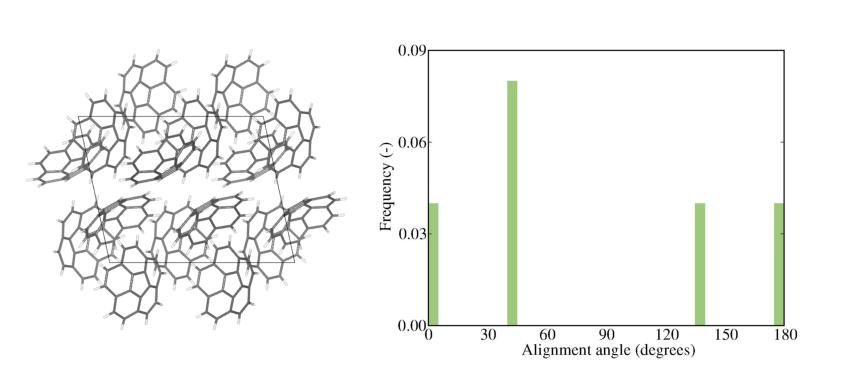
\includegraphics[width=0.65\linewidth]{Figures/corannulene_crystal.eps}
\caption{Snapshot of corannulene crystal structure (left) with alignment angle distribution (right).}
\label{figSI:corannulene_crystal}
\end{figure}
%

\subsection{Cut-off distance sensitivities}
The selection of the cut-off distance, $R$, influences the calculated average intermolecular distances, coordination numbers, and alignment angles.

Due to the molecular arrangements of the homogeneous corannulene clusters (that is, sandwich-type stacking is not present), these results are the most sensitive to the selection of $R$.


Figure \ref{figSI:alignmentangles_cutoffs} shows the alignment angle distributions for all homogeneous clusters using four different cut-off distances.  The influence of the cut-off distance is minimal in the 2pent15ring clusters, which show a very high proportion of molecules with at least one near neighbour at all cut-off distances.  At the higher cut-off distances, a second peak corresponding to further molecule layers (ie not the nearest neighbours alone) appears.  The corannulene clusters show relatively similar angle distributions across the cut-off distances, although the percent of molecules with a near neighbour increases dramatically between $R=0.5$ nm and $R=0.6$ nm.  
%
\begin{figure}[!tbh]
\centering
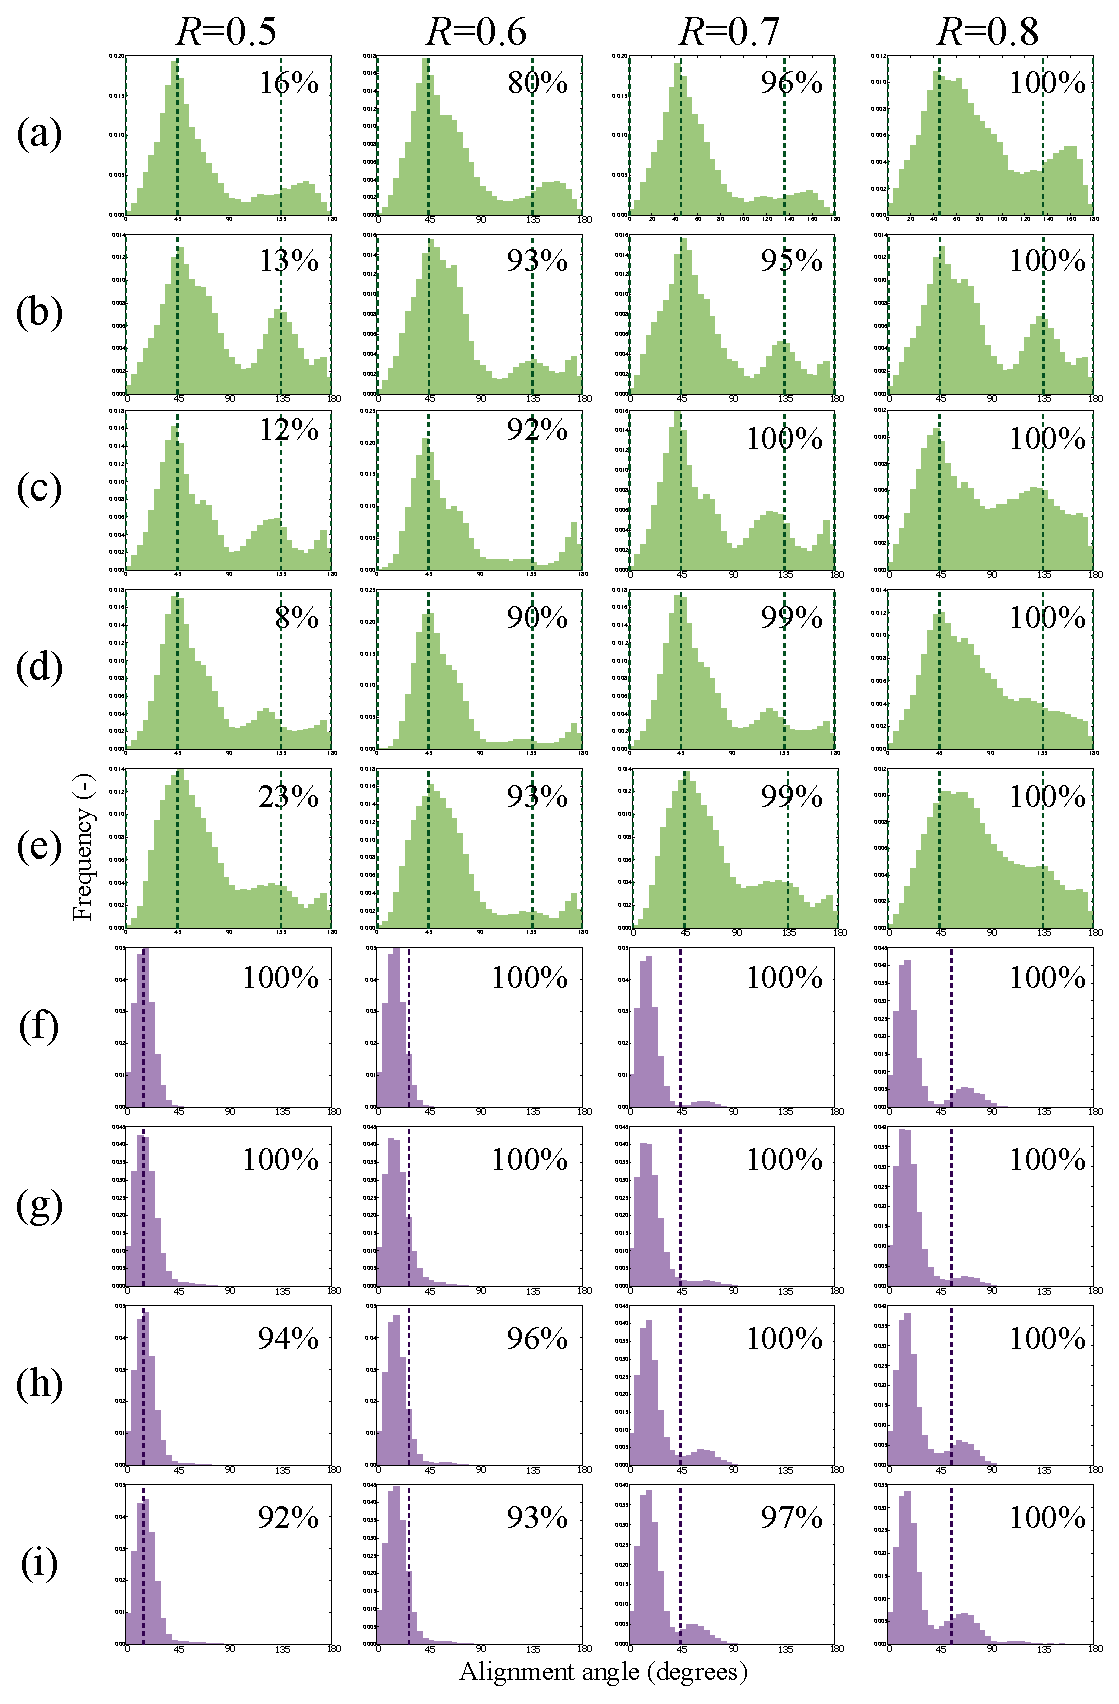
\includegraphics[width=1\linewidth]{Figures/AlignmentAnglesCutoffAssessment_SI.eps}
\caption{Alignment angle distributions at different cut-off distances, $R$, in nm for the following clusters: (a) ann\_25, (b) ann\_40, (c) ann\_50, (d) ann\_100, (e) ann\_200, (f) two\_25, (g) two\_40, (h) two\_50, (i) two\_100. Dashed lines correspond to the corannulene crystal structure (for (a)-(e)) and the minimised 2pent15ring dimer (for (f)-(i)). Percent values in the upper right hand corners of each angle distribution refer to the percent of molecules within the cluster that have at least one near neighbour.}
\label{figSI:alignmentangles_cutoffs}
\end{figure}
%

- Include figure of CN histograms with r=0.5 for corannulene and 2pent15ring

Note that for all systems, no neighbouring molecules are found using a cut-off distance of 0.4 nm or smaller (with the exception of ann\_40\_Kion\_1 and ann\_40\_Kion\_2 which have 15\% and 23\% of their molecules neighbouring at 0.4 nm).

- include table of intermolecular spacing for (just homo?) systems at different R values

Intuitively, for the corannulene molecule the cut-off distance selected correlates with the average intermolecular spacing between molecules (ie an increase in the cut-off distance produces an increase in the average intermolecular distance). %because increasing range of 'neighbours'
In contrast, the cut-off distance does not have a large impact on the average intermolecular spacing of homogeneous 2pent15ring molecules.  This highlights the highly stacked configuration of these molecules.



\subsection{Alignment angles - 100 molecule systems}
%
\begin{figure}[!tbh]
\centering
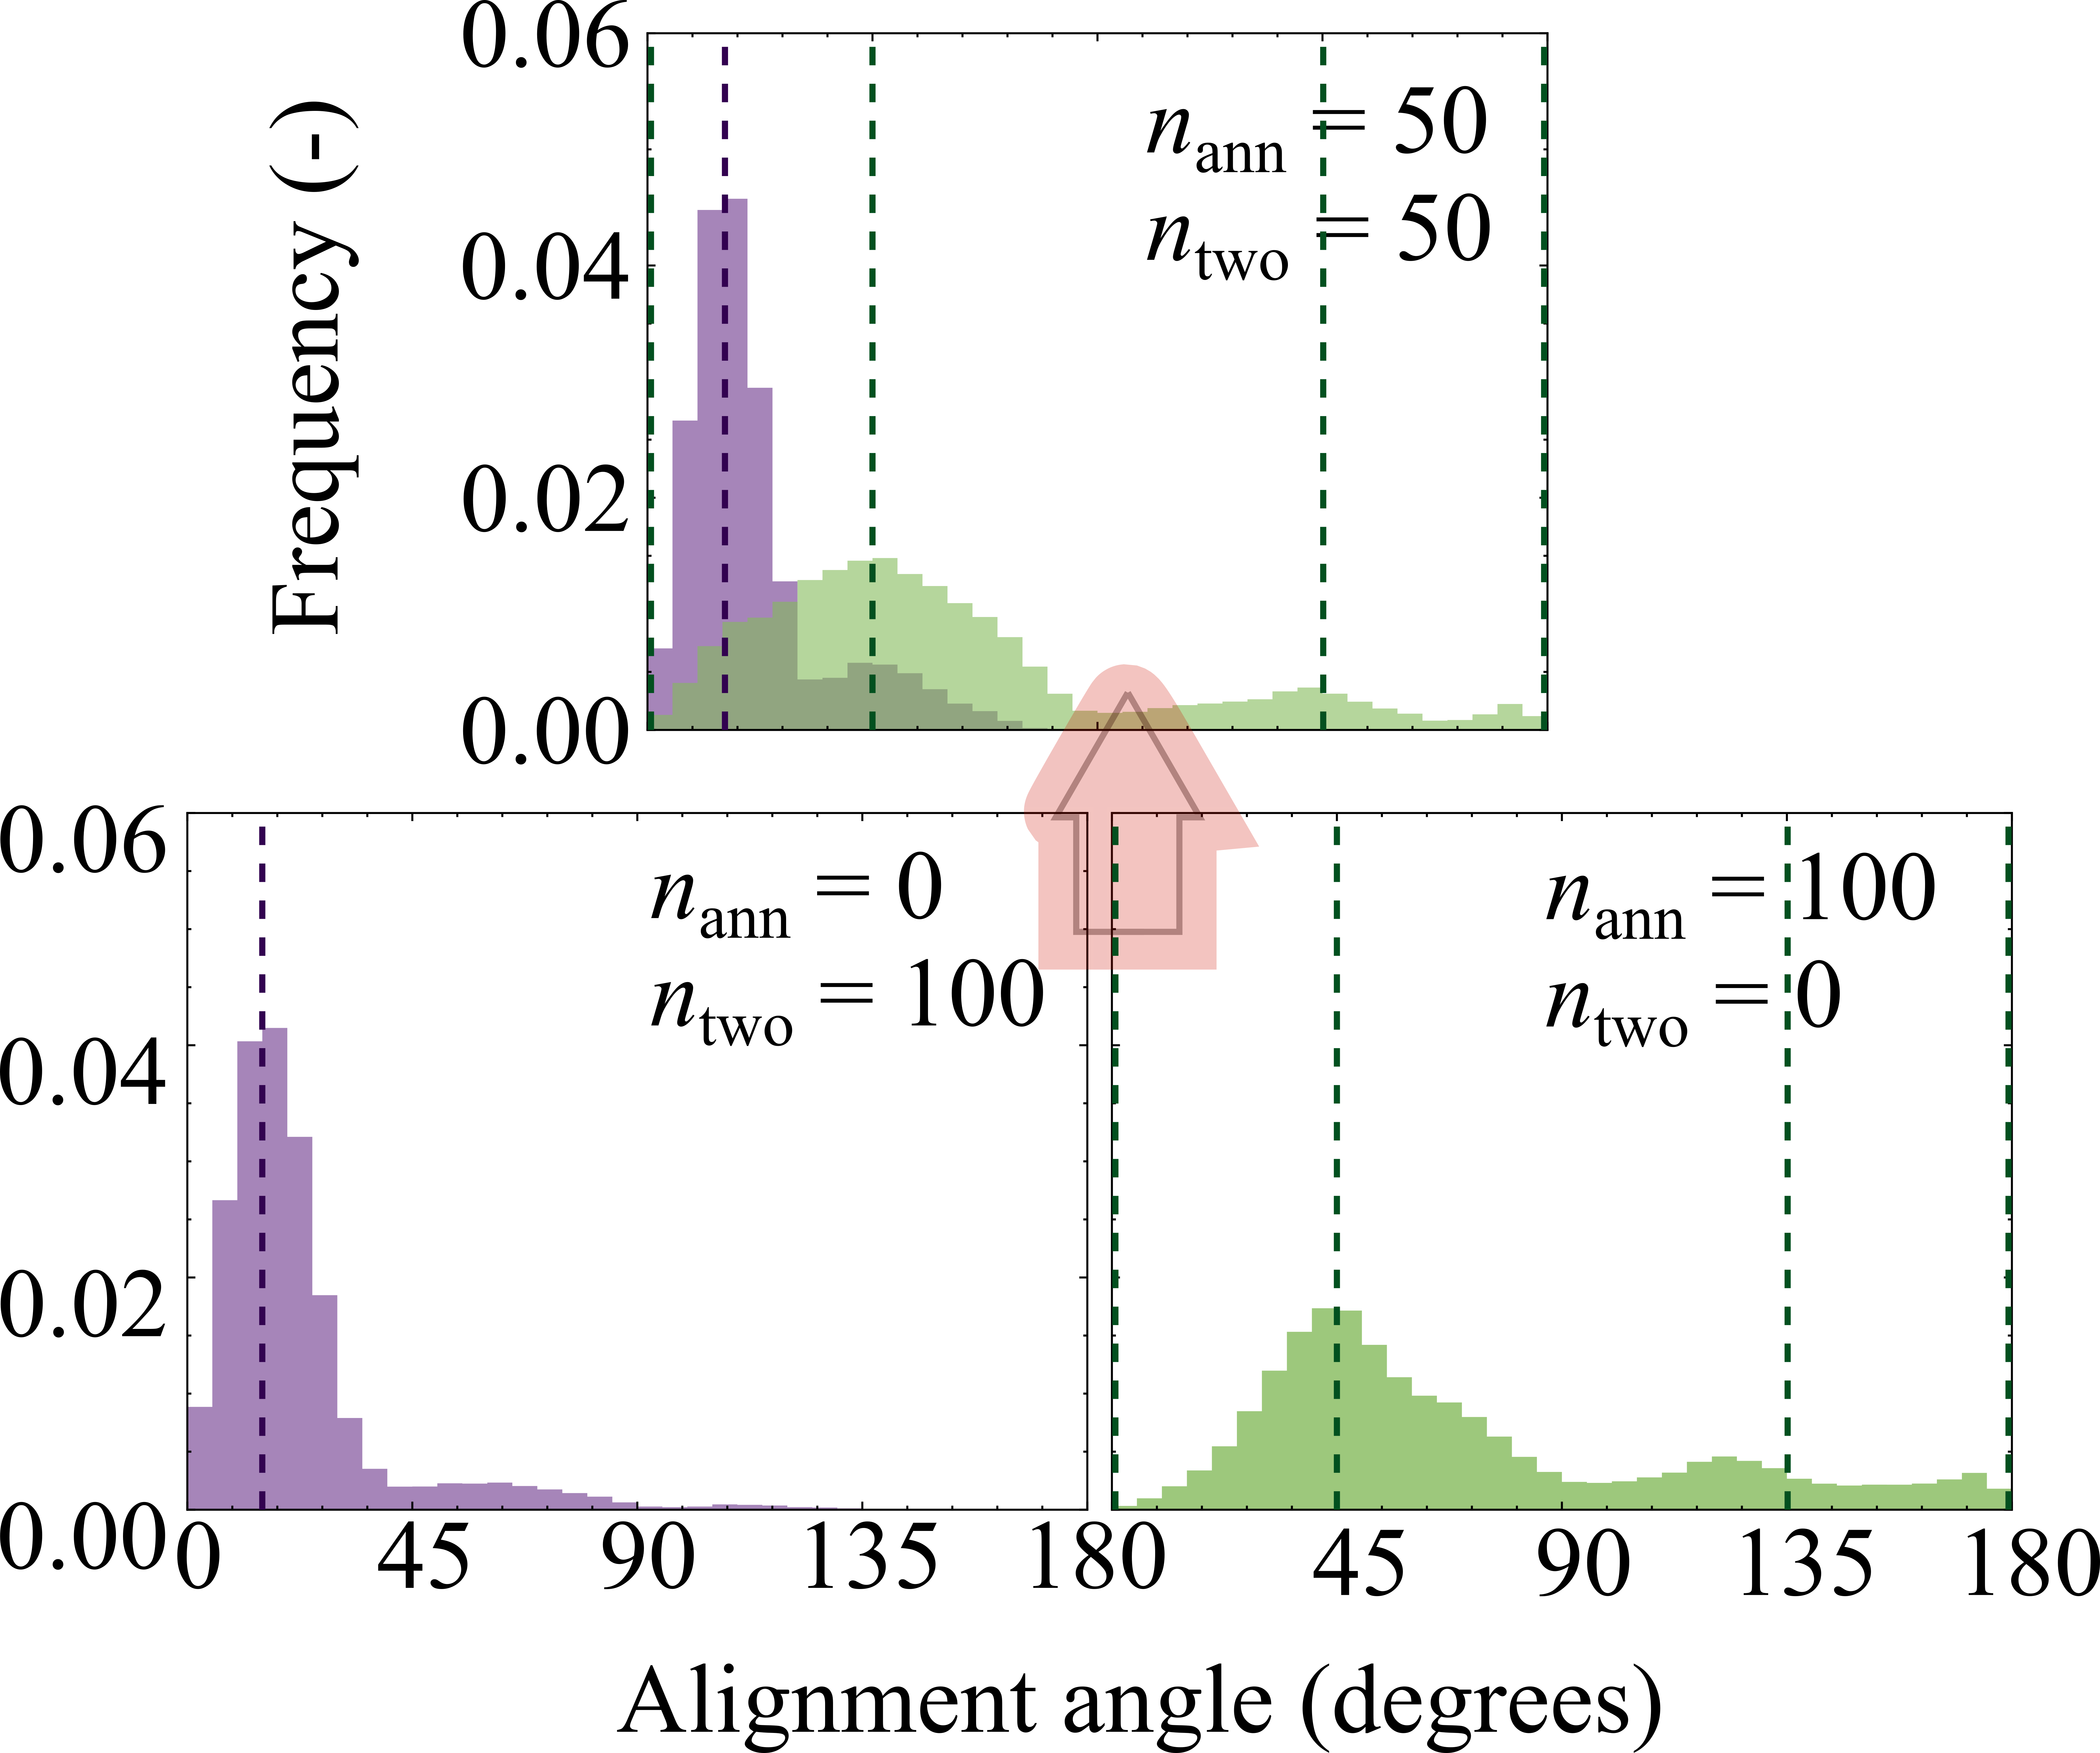
\includegraphics[width=0.5\linewidth]{Figures/alignment_angle_hetero_SI_draft.png}
\caption{Alignment angle distributions for homogeneous and heterogeneous 2pent15ring and corannulene clusters each containing 100 molecules.}
\label{figSI:alignmentangles_hetero}
\end{figure}
%

\subsection{Radial distances - homogeneous clusters}
For the homogeneous cases, the two molecule types show similar equilibrium radial distances according to the cluster diameter.


\newpage